\documentclass[xcolor=dvipsnames]{beamer}\usepackage[]{graphicx}\usepackage[]{color}
%% maxwidth is the original width if it is less than linewidth
%% otherwise use linewidth (to make sure the graphics do not exceed the margin)
\makeatletter
\def\maxwidth{ %
  \ifdim\Gin@nat@width>\linewidth
    \linewidth
  \else
    \Gin@nat@width
  \fi
}
\makeatother

\definecolor{fgcolor}{rgb}{0.345, 0.345, 0.345}
\newcommand{\hlnum}[1]{\textcolor[rgb]{0.686,0.059,0.569}{#1}}%
\newcommand{\hlstr}[1]{\textcolor[rgb]{0.192,0.494,0.8}{#1}}%
\newcommand{\hlcom}[1]{\textcolor[rgb]{0.678,0.584,0.686}{\textit{#1}}}%
\newcommand{\hlopt}[1]{\textcolor[rgb]{0,0,0}{#1}}%
\newcommand{\hlstd}[1]{\textcolor[rgb]{0.345,0.345,0.345}{#1}}%
\newcommand{\hlkwa}[1]{\textcolor[rgb]{0.161,0.373,0.58}{\textbf{#1}}}%
\newcommand{\hlkwb}[1]{\textcolor[rgb]{0.69,0.353,0.396}{#1}}%
\newcommand{\hlkwc}[1]{\textcolor[rgb]{0.333,0.667,0.333}{#1}}%
\newcommand{\hlkwd}[1]{\textcolor[rgb]{0.737,0.353,0.396}{\textbf{#1}}}%

\usepackage{framed}
\makeatletter
\newenvironment{kframe}{%
 \def\at@end@of@kframe{}%
 \ifinner\ifhmode%
  \def\at@end@of@kframe{\end{minipage}}%
  \begin{minipage}{\columnwidth}%
 \fi\fi%
 \def\FrameCommand##1{\hskip\@totalleftmargin \hskip-\fboxsep
 \colorbox{shadecolor}{##1}\hskip-\fboxsep
     % There is no \\@totalrightmargin, so:
     \hskip-\linewidth \hskip-\@totalleftmargin \hskip\columnwidth}%
 \MakeFramed {\advance\hsize-\width
   \@totalleftmargin\z@ \linewidth\hsize
   \@setminipage}}%
 {\par\unskip\endMakeFramed%
 \at@end@of@kframe}
\makeatother

\definecolor{shadecolor}{rgb}{.97, .97, .97}
\definecolor{messagecolor}{rgb}{0, 0, 0}
\definecolor{warningcolor}{rgb}{1, 0, 1}
\definecolor{errorcolor}{rgb}{1, 0, 0}
\newenvironment{knitrout}{}{} % an empty environment to be redefined in TeX

\usepackage{alltt}
\usetheme{Boadilla}
\usecolortheme[named=CornflowerBlue]{structure}
\usepackage{graphicx}
\usepackage{breqn}
\usepackage{xcolor}
\usepackage{booktabs}
\usepackage{verbatim}
\usepackage{tikz}
\usepackage{lmodern}
\usetikzlibrary{shadows,arrows,positioning}
\definecolor{links}{HTML}{2A1B81}
\hypersetup{colorlinks,linkcolor=links,urlcolor=links}
\usepackage{pgfpages}

\tikzstyle{block} = [rectangle, draw, text width=9em, text centered, rounded corners, minimum height=3em, minimum width=7em, top color = white, bottom color=brown!30,  drop shadow]

\newcommand{\ShowSexpr}[1]{\texttt{{\char`\\}Sexpr\{#1\}}}

\newcommand{\Bigtxt}[1]{\textbf{\textit{#1}}}
\IfFileExists{upquote.sty}{\usepackage{upquote}}{}
\begin{document}

\title[SWMPr overview, retrieve, and organize]{SWMPr overview, retrieve, and organize}

\author[M. Beck, T. O'Brien]{Marcus W. Beck\inst{1} \and Todd D. O'Brien\inst{2}}

\date{}

\institute[]{\inst{1} ORISE, USEPA NHEERL Gulf Ecology Division\\ Email: \href{mailto:beck.marcus@epa.gov}{beck.marcus@epa.gov} \and \inst{2} NOAA/NMFS COPEPOD Project\\ Email: \href{todd.obrien@noaa.gov}{todd.obrien@noaa.gov}}

% knitr setup


% load SWMPr from local


%%%%%%
\begin{frame}
\vspace{0.3in}
\centerline{
\begin{tikzpicture}
  \node[drop shadow={shadow xshift=0ex,shadow yshift=0ex},fill=white,draw] at (0,0) {
\includegraphics[width=0.9\textwidth]{imgs/workshop_logo.png}};
\end{tikzpicture}}
\titlepage
\end{frame}

%%%%%%
\begin{frame}{Objectives for the session}
\begin{itemize}
\item Why and what is SWMPr?\\~\\
\item How can data get from CDMO into R using SWMPr? \\~\\
\item What is the basic structure of a \texttt{swmpr} data object?\\~\\
\item What is data organization and how can SWMPr help?
\end{itemize}
\end{frame}

%%%%%%
\begin{frame}{Interactive portion}
\onslide<+->
We will use the swmpr1.Rproj project for this session, double-click to open in RStudio \\~\\
\begin{itemize}
\item location on flash drive\\~\\
\item location online \\~\\
\end{itemize}
\onslide<+->
You will run examples whenever you see this guy: \\~\\
\centerline{
\includegraphics[width = 0.15\textwidth]{imgs/swmprat.png}} 
Don't forget to use your stickies: {\color{green} green} for done/ok, {\color{red} red} for problem
\end{frame}

%%%%%%
\begin{frame}{Why and what is SWMPr?}
SWMP - System Wide Monitoring Program, initiated in 1995 to provide continuous monitoring data at over 300 stations in 28 US estuaries \\~\\
\centerline{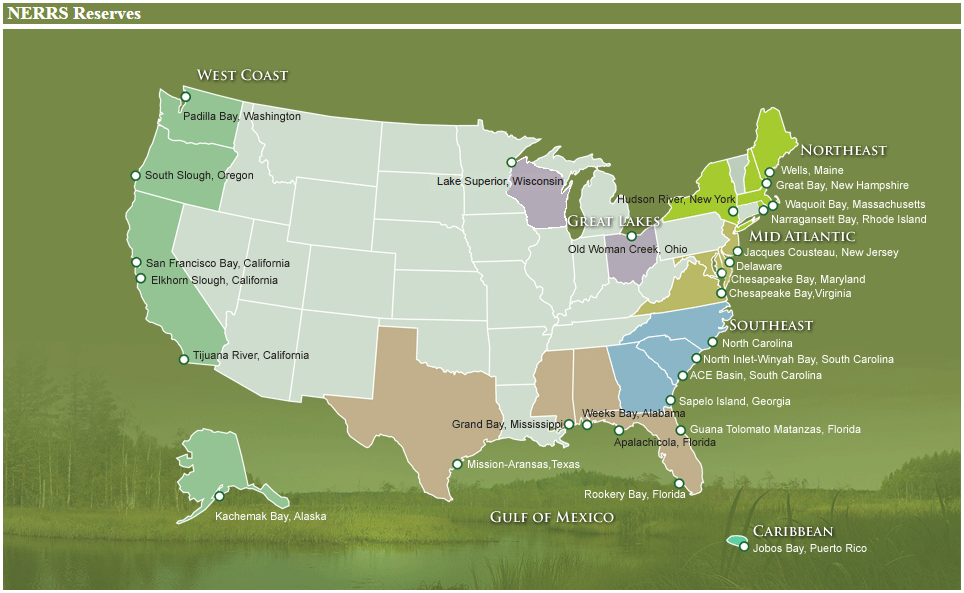
\includegraphics[width = 0.8\textwidth]{imgs/NERRS_locations.png}}
\tiny
\flushright
\href{http://nerrs.noaa.gov/ReservesMap.aspx}{http://nerrs.noaa.gov/ReservesMap.aspx}
\end{frame}

%%%%%%
\begin{frame}[t]{Why and what is SWMPr?}
CDMO (\href{http://cdmo.baruch.sc.edu/}{link}) is your one-stop shop for retrieving SWMP data \\~\\
\centerline{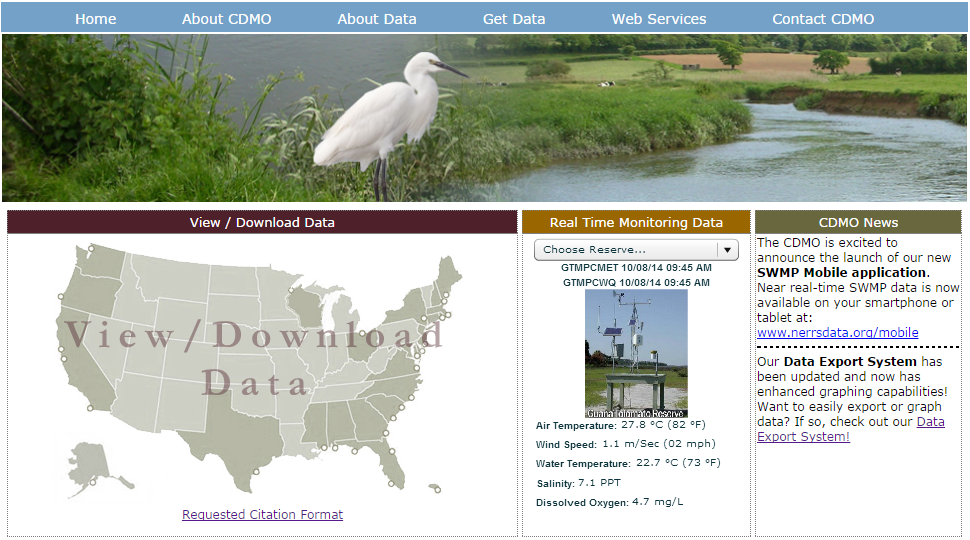
\includegraphics[width = \textwidth]{imgs/cdmo_front.png}}
\end{frame}

%%%%%%
\begin{frame}{Why and what is SWMPr?}
The raw data will look like this...\\~\\
\centerline{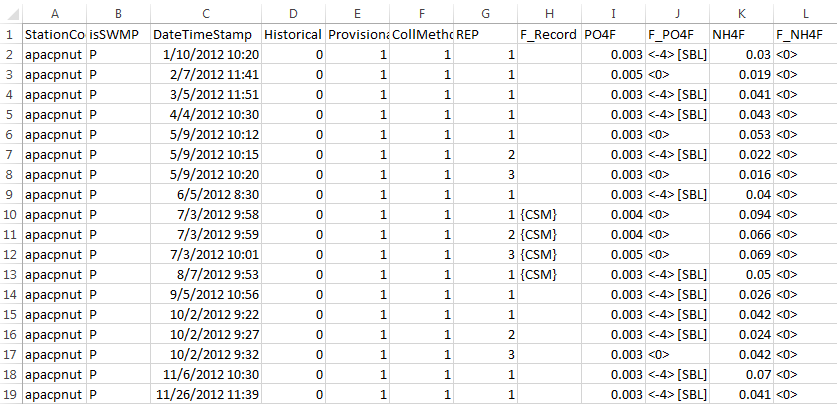
\includegraphics[width = 0.9\textwidth]{imgs/qaqc_ex.png}}
\end{frame}

%%%%%%
\begin{frame}[t]{Why and what is SWMPr?}
\onslide<+->
What are the challenges for evaluating SWMP data? \\~\\
\onslide<+->
\begin{itemize}
\item Knowing what we want \\~\\
\item Dealing with QAQC columns and removing `bad' observations \\~\\
\item Data we don't want... extra columns or irrelevant parameters \\~\\
\item Combining data for comparison\\~\\
\item Issues inherent with time series, e.g., missing data \\~\\
\item Others?
\end{itemize}
\end{frame}

%%%%%%
\begin{frame}{Why and what is SWMPr?}
\onslide<+->
\centerline{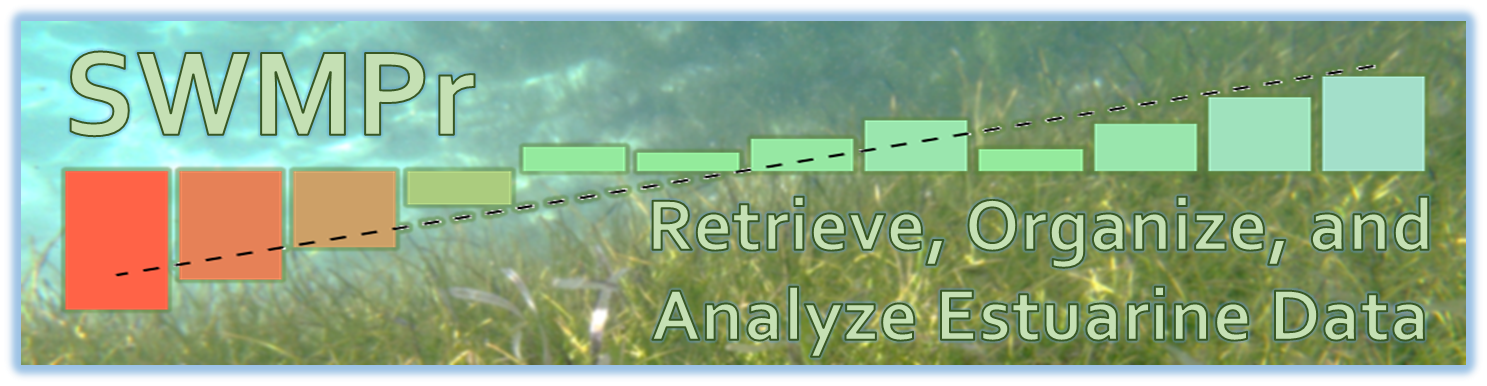
\includegraphics[width = 0.8\textwidth]{imgs/swmpr_logo.png}}
\vspace{0.2in}
\textbf{\emph{What}}: An R package to \Bigtxt{augment} existing CDMO services and to provide a \Bigtxt{bridge} to analysis\\~\\
\onslide<+->
\Bigtxt{Why}: There are many challenges working with SWMP data... a toolkit for addressing these challenges will be useful \\~\\
\onslide<+->
\Bigtxt{How}: Use the SWMPr functions to \Bigtxt{retrieve}, \Bigtxt{organize}, and \Bigtxt{analyze} SWMP data 
\end{frame}

%%%%%%
\begin{frame}[fragile]{Why and what is SWMPr?}
Some housekeeping...
\begin{knitrout}\scriptsize
\definecolor{shadecolor}{rgb}{0.969, 0.969, 0.969}\color{fgcolor}\begin{kframe}
\begin{alltt}
\hlcom{# install from CRAN (only do once)}
\hlkwd{install.packages}\hlstd{(}\hlstr{'SWMPr'}\hlstd{)}

\hlcom{# load for your current session}
\hlkwd{library}\hlstd{(SWMPr)}
\end{alltt}
\end{kframe}
\end{knitrout}
\url{https://cran.r-project.org/web/packages/SWMPr/index.html}
\end{frame}

%%%%%%
\begin{frame}[fragile]{Why and what is SWMPr? 
\includegraphics[width = 0.065\textwidth]{imgs/swmprat.png}}
\onslide<+->
Uses an \Bigtxt{object-oriented} structure... data are imported into R as a \texttt{swmpr} data object, with functions built to use this object\\~\\
What are the \Bigtxt{retrieve}, \Bigtxt{organize}, and \Bigtxt{analyze} functions? \\~\\
Run this code one line at a time... What comes up?
\begin{knitrout}\scriptsize
\definecolor{shadecolor}{rgb}{0.969, 0.969, 0.969}\color{fgcolor}\begin{kframe}
\begin{alltt}
\hlkwd{help.search}\hlstd{(}\hlstr{'retrieve'}\hlstd{,} \hlkwc{package} \hlstd{=} \hlstr{'SWMPr'}\hlstd{)}
\hlkwd{help.search}\hlstd{(}\hlstr{'organize'}\hlstd{,} \hlkwc{package} \hlstd{=} \hlstr{'SWMPr'}\hlstd{)}
\hlkwd{help.search}\hlstd{(}\hlstr{'analyze'}\hlstd{,} \hlkwc{package} \hlstd{=} \hlstr{'SWMPr'}\hlstd{)}
\end{alltt}
\end{kframe}
\end{knitrout}
\onslide<+->
What about this?
\begin{knitrout}\scriptsize
\definecolor{shadecolor}{rgb}{0.969, 0.969, 0.969}\color{fgcolor}\begin{kframe}
\begin{alltt}
\hlopt{?}\hlstd{import_local}
\end{alltt}
\end{kframe}
\end{knitrout}
Any useful information?
\end{frame}

%%%%%%
\begin{frame}[fragile]{Getting SWMP data into R}
Let's get some data into R!\\~\\
The \Bigtxt{retrieval} functions do two things: \\~\\
\begin{columns}[t]
\begin{column}{0.4\textwidth}
Import data directly from the CDMO:
\begin{knitrout}\scriptsize
\definecolor{shadecolor}{rgb}{0.969, 0.969, 0.969}\color{fgcolor}\begin{kframe}
\begin{alltt}
\hlstd{all_params}
\hlstd{all_params_dtrng}
\hlstd{single_param}
\hlstd{site_codes}
\hlstd{site_codes_ind}
\end{alltt}
\end{kframe}
\end{knitrout}
These functions require \href{http://cdmo.baruch.sc.edu/webservices.cfm}{registering your IP address}  with CDMO
\end{column}
\begin{column}{0.4\textwidth}
Import data from a local path:
\begin{knitrout}\scriptsize
\definecolor{shadecolor}{rgb}{0.969, 0.969, 0.969}\color{fgcolor}\begin{kframe}
\begin{alltt}
\hlstd{import_local}
\end{alltt}
\end{kframe}
\end{knitrout}
Imports data obtained from (and only from) the \href{http://cdmo.baruch.sc.edu/aqs/zips.cfm}{zip downloads} feature
\end{column}
\end{columns}
\end{frame}

%%%%%%
\begin{frame}[fragile]{Getting SWMP data into R 
\includegraphics[width = 0.065\textwidth]{imgs/swmprat.png}}
\onslide<+->
The `zip\_ex` folder in the project is a sample dataset that looks exactly like a folder you get from CDMO \\~\\
Let's import some data from that folder...
\begin{knitrout}\scriptsize
\definecolor{shadecolor}{rgb}{0.969, 0.969, 0.969}\color{fgcolor}\begin{kframe}
\begin{alltt}
\hlcom{# get data for apacpwq, all years}

\hlcom{# location of data}
\hlstd{mypath} \hlkwb{<-} \hlstr{'zip_ex'}

\hlcom{# import and assign to 'dat'}
\hlstd{dat} \hlkwb{<-} \hlkwd{import_local}\hlstd{(mypath,} \hlstr{'apacpwq'}\hlstd{,} \hlkwc{trace} \hlstd{= T)}
\end{alltt}
\end{kframe}
\end{knitrout}
\onslide<+->
What about this?
\begin{knitrout}\scriptsize
\definecolor{shadecolor}{rgb}{0.969, 0.969, 0.969}\color{fgcolor}\begin{kframe}
\begin{alltt}
\hlstd{dat2} \hlkwb{<-} \hlkwd{import_local}\hlstd{(mypath,} \hlstr{'apacp2012'}\hlstd{,} \hlkwc{trace} \hlstd{= T)}
\hlstd{dat3} \hlkwb{<-} \hlkwd{import_local}\hlstd{(mypath,} \hlstr{'apadbnut'}\hlstd{,} \hlkwc{trace} \hlstd{= T)}
\end{alltt}
\end{kframe}
\end{knitrout}

\end{frame}

%%%%%%
\begin{frame}[fragile]{Structure of the \texttt{swmpr} data object 
\includegraphics[width = 0.065\textwidth]{imgs/swmprat.png}}
\onslide<+->
Now we have data in our `workspace' that we can organize/analyze \\~\\
Try running the following...
\begin{knitrout}\scriptsize
\definecolor{shadecolor}{rgb}{0.969, 0.969, 0.969}\color{fgcolor}\begin{kframe}
\begin{alltt}
\hlkwd{head}\hlstd{(dat)}
\hlkwd{tail}\hlstd{(dat)}
\hlkwd{View}\hlstd{(dat)}
\hlkwd{str}\hlstd{(dat)}
\hlkwd{attributes}\hlstd{(dat)}
\end{alltt}
\end{kframe}
\end{knitrout}
\onslide<+->
How are the data organized?  \\~\\
What are the column names? \\~\\
What are the attributes?
\end{frame}

%%%%%%
\begin{frame}[fragile, shrink]{Structure of the \texttt{swmpr} data object}
The \texttt{swmpr} object is a \texttt{data.frame} and a list of attributes 
\begin{knitrout}\scriptsize
\definecolor{shadecolor}{rgb}{0.969, 0.969, 0.969}\color{fgcolor}\begin{kframe}
\begin{alltt}
\hlkwd{head}\hlstd{(dat,} \hlnum{3}\hlstd{)}
\end{alltt}
\begin{verbatim}
##         datetimestamp temp f_temp spcond f_spcond sal f_sal do_pct f_do_pct
## 1 2011-01-01 00:00:00   11   <0>      44     <0>   28  <0>      68     <0> 
## 2 2011-01-01 00:15:00   11   <0>      44     <0>   28  <0>      68     <0> 
## 3 2011-01-01 00:30:00   11   <0>      44     <0>   28  <0>      68     <0> 
##   do_mgl f_do_mgl depth f_depth cdepth f_cdepth level f_level clevel f_clevel
## 1      6     <0>      2    <0>       2     <3>     NA   <-1>      NA       NA
## 2      6     <0>      2    <0>       2     <3>     NA   <-1>      NA       NA
## 3      6     <0>      2    <0>       2     <3>     NA   <-1>      NA       NA
##   ph f_ph turb f_turb chlfluor f_chlfluor
## 1  8 <0>     3   <0>        NA      <-1> 
## 2  8 <0>     3   <0>        NA      <-1> 
## 3  8 <0>     2   <0>        NA      <-1>
\end{verbatim}
\begin{alltt}
\hlkwd{names}\hlstd{(}\hlkwd{attributes}\hlstd{(dat))}
\end{alltt}
\begin{verbatim}
## [1] "names"       "row.names"   "class"       "station"     "parameters" 
## [6] "qaqc_cols"   "date_rng"    "timezone"    "stamp_class"
\end{verbatim}
\begin{alltt}
\hlkwd{attr}\hlstd{(dat,} \hlstr{'parameters'}\hlstd{)}
\end{alltt}
\begin{verbatim}
##  [1] "temp"     "spcond"   "sal"      "do_pct"   "do_mgl"   "depth"   
##  [7] "cdepth"   "level"    "clevel"   "ph"       "turb"     "chlfluor"
\end{verbatim}
\end{kframe}
\end{knitrout}
\end{frame}

%%%%%%
\begin{frame}[fragile]{Data organization with SWMPr}
First problem is solved... we know how to get SWMP data from CDMO into R: \\~\\
\begin{itemize}
\item Download a dataset from zip downloads \\~\\
\item Find where the data have downloaded \\~\\
\item Import using \texttt{import_local} \\~\\
\item Have a look at the data (\texttt{head}, \texttt{View}, \texttt{attributes}) \\~\\
\item Lost? Check the help files: \texttt{?import\_local}\\~\\
\end{itemize}
Now we can think about preprocessing or organizing prior to analysis
\end{frame}

%%%%%%
\begin{frame}[fragile]{Data organization with SWMPr}
Problem 1 solved... we know how to get SWMP data from CDMO into R: \\~\\
\begin{itemize}
\item Download a dataset from zip downloads \\~\\
\item Find where the data have downloaded \\~\\
\item Import using \texttt{import_local} \\~\\
\item Have a look at the data (\texttt{head}, \texttt{View}, \texttt{attributes}) \\~\\
\item Lost? Check the help files: \texttt{?import\_local}\\~\\
\end{itemize}
Now we can think about preprocessing or organizing prior to analysis
\end{frame}

%%%%%%
\begin{frame}[t]{Data organization with SWMPr}
\onslide<+->
What are the challenges for evaluating SWMP data? \\~\\
\onslide<+->
\begin{itemize}
\item Knowing what we want \\~\\
\item Dealing with QAQC columns and removing `bad' observations \\~\\
\item Data we don't want... extra columns or irrelevant parameters \\~\\
\item Combining data for comparison\\~\\
\item Issues inherent with time series, e.g., missing data \\~\\
\item Others?
\end{itemize}
\end{frame}

%%%%%%
\begin{frame}[fragile]{Data organization with SWMPr 
\includegraphics[width = 0.065\textwidth]{imgs/swmprat.png}}
\onslide<+->
Take a few minutes to acquaint yourself with the \Bigtxt{organize} functions:
\begin{knitrout}\scriptsize
\definecolor{shadecolor}{rgb}{0.969, 0.969, 0.969}\color{fgcolor}\begin{kframe}
\begin{alltt}
\hlkwd{help.search}\hlstd{(}\hlstr{'organize'}\hlstd{,} \hlkwc{package} \hlstd{=} \hlstr{'SWMPr'}\hlstd{)}
\end{alltt}
\end{kframe}
\end{knitrout}
\onslide<+->
Which function would you use first? \\~\\
Which would you use to reduce data volume or select certain variables? \\~\\
Can any be used to combine \texttt{swmpr} data objects? 
\end{frame}

%%%%%%
\begin{frame}[fragile]{Data organization with SWMPr 
\includegraphics[width = 0.065\textwidth]{imgs/swmprat.png}}
\onslide<+->
Perhaps you want to deal with QAQC columns first... \\~\\
From the zips folder, import all of the weather data for apaebmet (\texttt{?import\_local})
\onslide<+->
\begin{knitrout}\scriptsize
\definecolor{shadecolor}{rgb}{0.969, 0.969, 0.969}\color{fgcolor}\begin{kframe}
\begin{alltt}
\hlcom{# import data }
\hlstd{mypath} \hlkwb{<-} \hlstr{'zip_ex'}
\hlstd{dat} \hlkwb{<-} \hlkwd{import_local}\hlstd{(mypath,} \hlstr{'apaebmet'}\hlstd{)}
\end{alltt}
\end{kframe}
\end{knitrout}
\onslide<+->
View the data, what are the columns? \\~\\
Try running \texttt{qaqc} (\texttt{?qaqc}) and view again, what happened?
\onslide<+->
\begin{knitrout}\scriptsize
\definecolor{shadecolor}{rgb}{0.969, 0.969, 0.969}\color{fgcolor}\begin{kframe}
\begin{alltt}
\hlkwd{View}\hlstd{(dat)}
\hlstd{dat2} \hlkwb{<-} \hlkwd{qaqc}\hlstd{(dat)}
\hlkwd{View}\hlstd{(dat2)}
\end{alltt}
\end{kframe}
\end{knitrout}
\end{frame}

%%%%%%
\begin{frame}[fragile]{Data organization with SWMPr 
\includegraphics[width = 0.065\textwidth]{imgs/swmprat.png}}
\onslide<+->
Try playing with the \texttt{qaqc\_keep} argument (\texttt{?qaqc})... \\~\\
How are these different?
\onslide<+->
\begin{knitrout}\scriptsize
\definecolor{shadecolor}{rgb}{0.969, 0.969, 0.969}\color{fgcolor}\begin{kframe}
\begin{alltt}
\hlcom{# different options for qaqc}
\hlstd{dat2} \hlkwb{<-} \hlkwd{qaqc}\hlstd{(dat)}
\hlstd{dat3} \hlkwb{<-} \hlkwd{qaqc}\hlstd{(dat,} \hlkwc{qaqc_keep} \hlstd{=} \hlkwd{c}\hlstd{(}\hlstr{'0'}\hlstd{,} \hlstr{'-1'}\hlstd{))}
\hlstd{dat4} \hlkwb{<-} \hlkwd{qaqc}\hlstd{(dat,} \hlkwc{qaqc_keep} \hlstd{=} \hlkwa{NULL}\hlstd{)}
\hlstd{dat5} \hlkwb{<-} \hlkwd{qaqc}\hlstd{(dat,} \hlkwc{qaqc_keep} \hlstd{=} \hlstr{'CSM'}\hlstd{)}
\end{alltt}
\end{kframe}
\end{knitrout}
Changes are hard to visualize for lots of data - as a proof of concept, try running \texttt{qaqcchk} on any of the datasets 
\begin{knitrout}\scriptsize
\definecolor{shadecolor}{rgb}{0.969, 0.969, 0.969}\color{fgcolor}\begin{kframe}
\begin{alltt}
\hlkwd{qaqcchk}\hlstd{(dat)}
\hlkwd{qaqcchk}\hlstd{(dat2)}
\hlkwd{qaqcchk}\hlstd{(dat3)}
\hlkwd{qaqcchk}\hlstd{(dat4)}
\hlkwd{qaqcchk}\hlstd{(dat5)}
\end{alltt}
\end{kframe}
\end{knitrout}
\end{frame}

%%%%%%
\begin{frame}[fragile]{Data organization with SWMPr 
\includegraphics[width = 0.065\textwidth]{imgs/swmprat.png}} 
\onslide<+->
We'll continue with the water quality data for apawq - import again and run the \texttt{qaqc} function
\onslide<+->
\begin{knitrout}\scriptsize
\definecolor{shadecolor}{rgb}{0.969, 0.969, 0.969}\color{fgcolor}\begin{kframe}
\begin{alltt}
\hlcom{# import apawq}
\hlstd{mypath} \hlkwb{<-} \hlstr{'zip_ex'}
\hlstd{dat} \hlkwb{<-} \hlkwd{import_local}\hlstd{(mypath,} \hlstr{'apadbwq'}\hlstd{)}
\hlstd{dat} \hlkwb{<-} \hlkwd{qaqc}\hlstd{(dat)}
\end{alltt}
\end{kframe}
\end{knitrout}
\onslide<+->
What is the next logical step after dealing with QAQC values? \\~\\
How would we further want to organize the data? \\~\\
Maybe we want to subset the data... 
\begin{knitrout}\scriptsize
\definecolor{shadecolor}{rgb}{0.969, 0.969, 0.969}\color{fgcolor}\begin{kframe}
\begin{alltt}
\hlcom{# view help file}
\hlopt{?}\hlstd{subset.swmpr}
\end{alltt}
\end{kframe}
\end{knitrout}
\end{frame}

%%%%%%
\begin{frame}[fragile]{Data organization with SWMPr}
The \texttt{subset} function has several arguments (help file \texttt{?subset.swmpr})\\~\\
Not all are necessary for every task \\~\\
\begin{itemize}
\item \texttt{swmpr\_in}: input data (\texttt{swmpr} object)
\item \texttt{subset}: dates to keep
\item \texttt{select}: parameters to keep
\item \texttt{operator}: less than, greater than, etc. if only one date in subset
\item \texttt{rem\_rows}: remove empty rows
\item \texttt{rem\_cols}: remove empty columns \\~\\
\end{itemize}
\end{frame}

%%%%%%
\begin{frame}[fragile]{Data organization with SWMPr}
\onslide<+->
The \texttt{select} argument of \texttt{subset} is used to select parameters of interest - one to many
\begin{knitrout}\scriptsize
\definecolor{shadecolor}{rgb}{0.969, 0.969, 0.969}\color{fgcolor}\begin{kframe}
\begin{alltt}
\hlcom{# select the DO column}
\hlstd{tmp} \hlkwb{<-} \hlkwd{subset}\hlstd{(dat,} \hlkwc{select} \hlstd{=} \hlstr{'do_mgl'}\hlstd{)}
\hlkwd{head}\hlstd{(tmp)}
\end{alltt}
\begin{verbatim}
##         datetimestamp do_mgl
## 1 2011-01-01 00:00:00     NA
## 2 2011-01-01 00:15:00     NA
## 3 2011-01-01 00:30:00     NA
## 4 2011-01-01 00:45:00     NA
## 5 2011-01-01 01:00:00     NA
## 6 2011-01-01 01:15:00     NA
\end{verbatim}
\end{kframe}
\end{knitrout}
Selecting more than one column...
\onslide<+->
\begin{knitrout}\scriptsize
\definecolor{shadecolor}{rgb}{0.969, 0.969, 0.969}\color{fgcolor}\begin{kframe}
\begin{alltt}
\hlcom{# select DO and salinity}
\hlstd{tmp} \hlkwb{<-} \hlkwd{subset}\hlstd{(dat,} \hlkwc{select} \hlstd{=} \hlkwd{c}\hlstd{(}\hlstr{'do_mgl'}\hlstd{,} \hlstr{'sal'}\hlstd{))}
\hlkwd{head}\hlstd{(tmp)}
\end{alltt}
\end{kframe}
\end{knitrout}
\end{frame}

%%%%%%
\begin{frame}[fragile]{Data organization with SWMPr}
The \texttt{subset} argument of \texttt{subset.swmpr} selects a date range \\~\\
The dates must have a specific format: `YYYY-mm-dd HH:MM'
\begin{knitrout}\scriptsize
\definecolor{shadecolor}{rgb}{0.969, 0.969, 0.969}\color{fgcolor}\begin{kframe}
\begin{alltt}
\hlcom{# select a date range, July 2012}
\hlstd{dates} \hlkwb{<-} \hlkwd{c}\hlstd{(}\hlstr{'2012-07-01 12:00'}\hlstd{,} \hlstr{'2012-07-31 6:30'}\hlstd{)}
\hlstd{tmp} \hlkwb{<-} \hlkwd{subset}\hlstd{(dat,} \hlkwc{subset} \hlstd{= dates)}
\hlkwd{head}\hlstd{(tmp)} \hlcom{# view first six rows}
\end{alltt}
\begin{verbatim}
##         datetimestamp temp spcond sal do_pct do_mgl depth cdepth level clevel
## 1 2012-07-01 12:00:00   NA     50  33    104      7     2     NA    NA     NA
## 2 2012-07-01 12:15:00   NA     50  33    101      7     2     NA    NA     NA
## 3 2012-07-01 12:30:00   NA     50  33    104      7     2     NA    NA     NA
## 4 2012-07-01 12:45:00   NA     50  33    104      7     2     NA    NA     NA
## 5 2012-07-01 13:00:00   NA     50  33    104      7     2     NA    NA     NA
## 6 2012-07-01 13:15:00   NA     52  34    104      7     2     NA    NA     NA
##   ph turb chlfluor
## 1  8    3       NA
## 2  8   11       NA
## 3  8    8       NA
## 4  8   10       NA
## 5  8   15       NA
## 6  8   12       NA
\end{verbatim}
\end{kframe}
\end{knitrout}
\end{frame}


%%%%%%
\begin{frame}[fragile]{Data organization with SWMPr 
\includegraphics[width = 0.065\textwidth]{imgs/swmprat.png}}
\begin{itemize}
\item \onslide<1->
Import the weather data at apaeb
\onslide<2->
\begin{knitrout}\scriptsize
\definecolor{shadecolor}{rgb}{0.969, 0.969, 0.969}\color{fgcolor}\begin{kframe}
\begin{alltt}
\hlstd{mypath} \hlkwb{<-} \hlstr{'zip_ex'}
\hlstd{dat} \hlkwb{<-} \hlkwd{import_local}\hlstd{(mypath,} \hlstr{'apaebmet'}\hlstd{)}
\end{alltt}
\end{kframe}
\end{knitrout}
\vspace{0.1in}
\item \onslide<1->
Deal with QAQC columns
\onslide<3->
\begin{knitrout}\scriptsize
\definecolor{shadecolor}{rgb}{0.969, 0.969, 0.969}\color{fgcolor}\begin{kframe}
\begin{alltt}
\hlstd{tmp} \hlkwb{<-} \hlkwd{qaqc}\hlstd{(dat)}
\end{alltt}
\end{kframe}
\end{knitrout}
\vspace{0.1in}
\item \onslide<1->
Select two columns of interest
\onslide<4->
\begin{knitrout}\scriptsize
\definecolor{shadecolor}{rgb}{0.969, 0.969, 0.969}\color{fgcolor}\begin{kframe}
\begin{alltt}
\hlstd{tmp} \hlkwb{<-} \hlkwd{subset}\hlstd{(tmp,} \hlkwc{select} \hlstd{=} \hlkwd{c}\hlstd{(}\hlstr{'temp'}\hlstd{,} \hlstr{'wind'}\hlstd{))}
\end{alltt}
\end{kframe}
\end{knitrout}
\vspace{0.1in}
\item \onslide<1->
Subset a date range
\onslide<5->
\begin{knitrout}\scriptsize
\definecolor{shadecolor}{rgb}{0.969, 0.969, 0.969}\color{fgcolor}\begin{kframe}
\begin{alltt}
\hlstd{dates} \hlkwb{<-} \hlkwd{c}\hlstd{(}\hlstr{'2012-01-01 0:0'}\hlstd{,} \hlstr{'2012-01-31 0:0'}\hlstd{)}
\hlstd{tmp} \hlkwb{<-} \hlkwd{subset}\hlstd{(tmp,} \hlkwc{subset} \hlstd{= dates)}
\end{alltt}
\end{kframe}
\end{knitrout}
\end{itemize}
\end{frame}

%%%%%%
\begin{frame}[fragile]{Data organization with SWMPr 
\includegraphics[width = 0.065\textwidth]{imgs/swmprat.png}}
\onslide<+->
Bonus: What if we want to select all values before or after a date?  \\~\\
See \texttt{?subset.swmpr}, requires the \texttt{operator} argument
\onslide<+->
\begin{knitrout}\scriptsize
\definecolor{shadecolor}{rgb}{0.969, 0.969, 0.969}\color{fgcolor}\begin{kframe}
\begin{alltt}
\hlcom{# get observations for 2013}
\hlstd{dates} \hlkwb{<-} \hlstr{'2013-01-01 00:00'}
\hlstd{tmp} \hlkwb{<-} \hlkwd{subset}\hlstd{(dat,} \hlkwc{subset} \hlstd{= dates,} \hlkwc{operator} \hlstd{=} \hlstr{'>='}\hlstd{)}
\hlkwd{head}\hlstd{(tmp)}
\end{alltt}
\end{kframe}
\end{knitrout}
\end{frame}

%%%%%%
\begin{frame}[fragile]{Data organization with SWMPr 
\includegraphics[width = 0.065\textwidth]{imgs/swmprat.png}}
\onslide<+->
A final nod to the \texttt{comb} and \texttt{setstep} functions \\~\\
Run the following, view the results, discuss with your neighbors:
\begin{knitrout}\scriptsize
\definecolor{shadecolor}{rgb}{0.969, 0.969, 0.969}\color{fgcolor}\begin{kframe}
\begin{alltt}
\hlstd{mypath} \hlkwb{<-} \hlstr{'zip_ex'}
\hlstd{dat_met} \hlkwb{<-} \hlkwd{import_local}\hlstd{(mypath,} \hlstr{'apaebmet'}\hlstd{)}
\hlstd{dat_met} \hlkwb{<-} \hlkwd{qaqc}\hlstd{(dat_met)}
\hlstd{dat_wq} \hlkwb{<-} \hlkwd{import_local}\hlstd{(mypath,} \hlstr{'apadbwq'}\hlstd{)}
\hlstd{dat_wq} \hlkwb{<-} \hlkwd{qaqc}\hlstd{(dat_wq)}

\hlcom{# what does this do?}
\hlstd{tmp1} \hlkwb{<-} \hlkwd{comb}\hlstd{(dat_wq, dat_met,} \hlkwc{timestep} \hlstd{=} \hlnum{120}\hlstd{)}
\end{alltt}
\end{kframe}
\end{knitrout}
\onslide<+->
Now try this...
\begin{knitrout}\scriptsize
\definecolor{shadecolor}{rgb}{0.969, 0.969, 0.969}\color{fgcolor}\begin{kframe}
\begin{alltt}
\hlstd{tmp2} \hlkwb{<-} \hlkwd{setstep}\hlstd{(dat_wq,} \hlkwc{timestep} \hlstd{=} \hlnum{60}\hlstd{)}
\end{alltt}
\end{kframe}
\end{knitrout}
\end{frame}

%%%%%%
\begin{frame}[fragile]{Summary}
Now you have an idea of how to organize SWMP data for analysis!\\~\\
Here's what we did: \\~\\
\begin{itemize}
\item \Bigtxt{Import} SWMP data into R
\item Evaluate and \Bigtxt{handle QAQC} flags in the data 
\item \Bigtxt{Subset} to select variables or time ranges of interest 
\item \Bigtxt{Combine} data for comparison or data simplification \\~\\
\end{itemize}
Consult the SWMP cookboook for an example workflow\\~\\
Check the help files for usage (reference manual on \href{https://cran.r-project.org/web/packages/SWMPr/index.html}{CRAN}) \\~\\
After break... what are some ways we can visualize or analyze the data?
\end{frame}

%%%%%%
\begin{frame}
\vspace{0.3in}
\centerline{
\begin{tikzpicture}
  \node[drop shadow={shadow xshift=0ex,shadow yshift=0ex},fill=white,draw] at (0,0) {
\includegraphics[width=0.9\textwidth]{imgs/workshop_logo.png}};
\end{tikzpicture}}
\vspace{0.5in}
\Large
\centerline{\Bigtxt{Questions??}}
\end{frame}

\end{document}
